\subsubsection{Obervabilidad y maniobrabilidad}

Cuando $N\to\infty$, siempre que contemos con distribuciones uniformes, es viable interpretar al enjambre como un continuo. Llamaremos $C$ al área que ocupa dicha geometría. Esta aproximación nos permitirá aplicar el teorema fundamental del cálculo, de modo que el sumatorio de (\ref{eq: l_sigma}) se convertirá en una integración a lo largo de toda la distribución:

\begin{align} \label{eq: l1_cont}
    L_\sigma^1(p_c, x) & = 
    \frac{1}{N D^2} \iint_C ||\nabla\sigma(p_c)|| \left(
    \begin{bmatrix}\cos(\theta) & \sin(\theta) \end{bmatrix} 
    \begin{bmatrix}x_i^X \\ x_i^Y \end{bmatrix}
    \right)
    \begin{bmatrix}x_i^X \\ x_i^Y \end{bmatrix} 
    \mathrm{d}X \mathrm{d}Y
    \nonumber\\
    & = \frac{1}{N D^2} \iint_C ||\nabla\sigma(p_c)||
    \begin{bmatrix}
        X^2 \cos(\theta) + XY\, \sin(\theta) \\
        Y^2 \sin(\theta) + XY\, \cos(\theta) \\
    \end{bmatrix}
    \mathrm{d}X \mathrm{d}Y,
\end{align}

donde $\theta$ es el ángulo que forma $\nabla\sigma(p_c)$ con respecto al eje X.

\begin{figure}[!h]
    \centering
    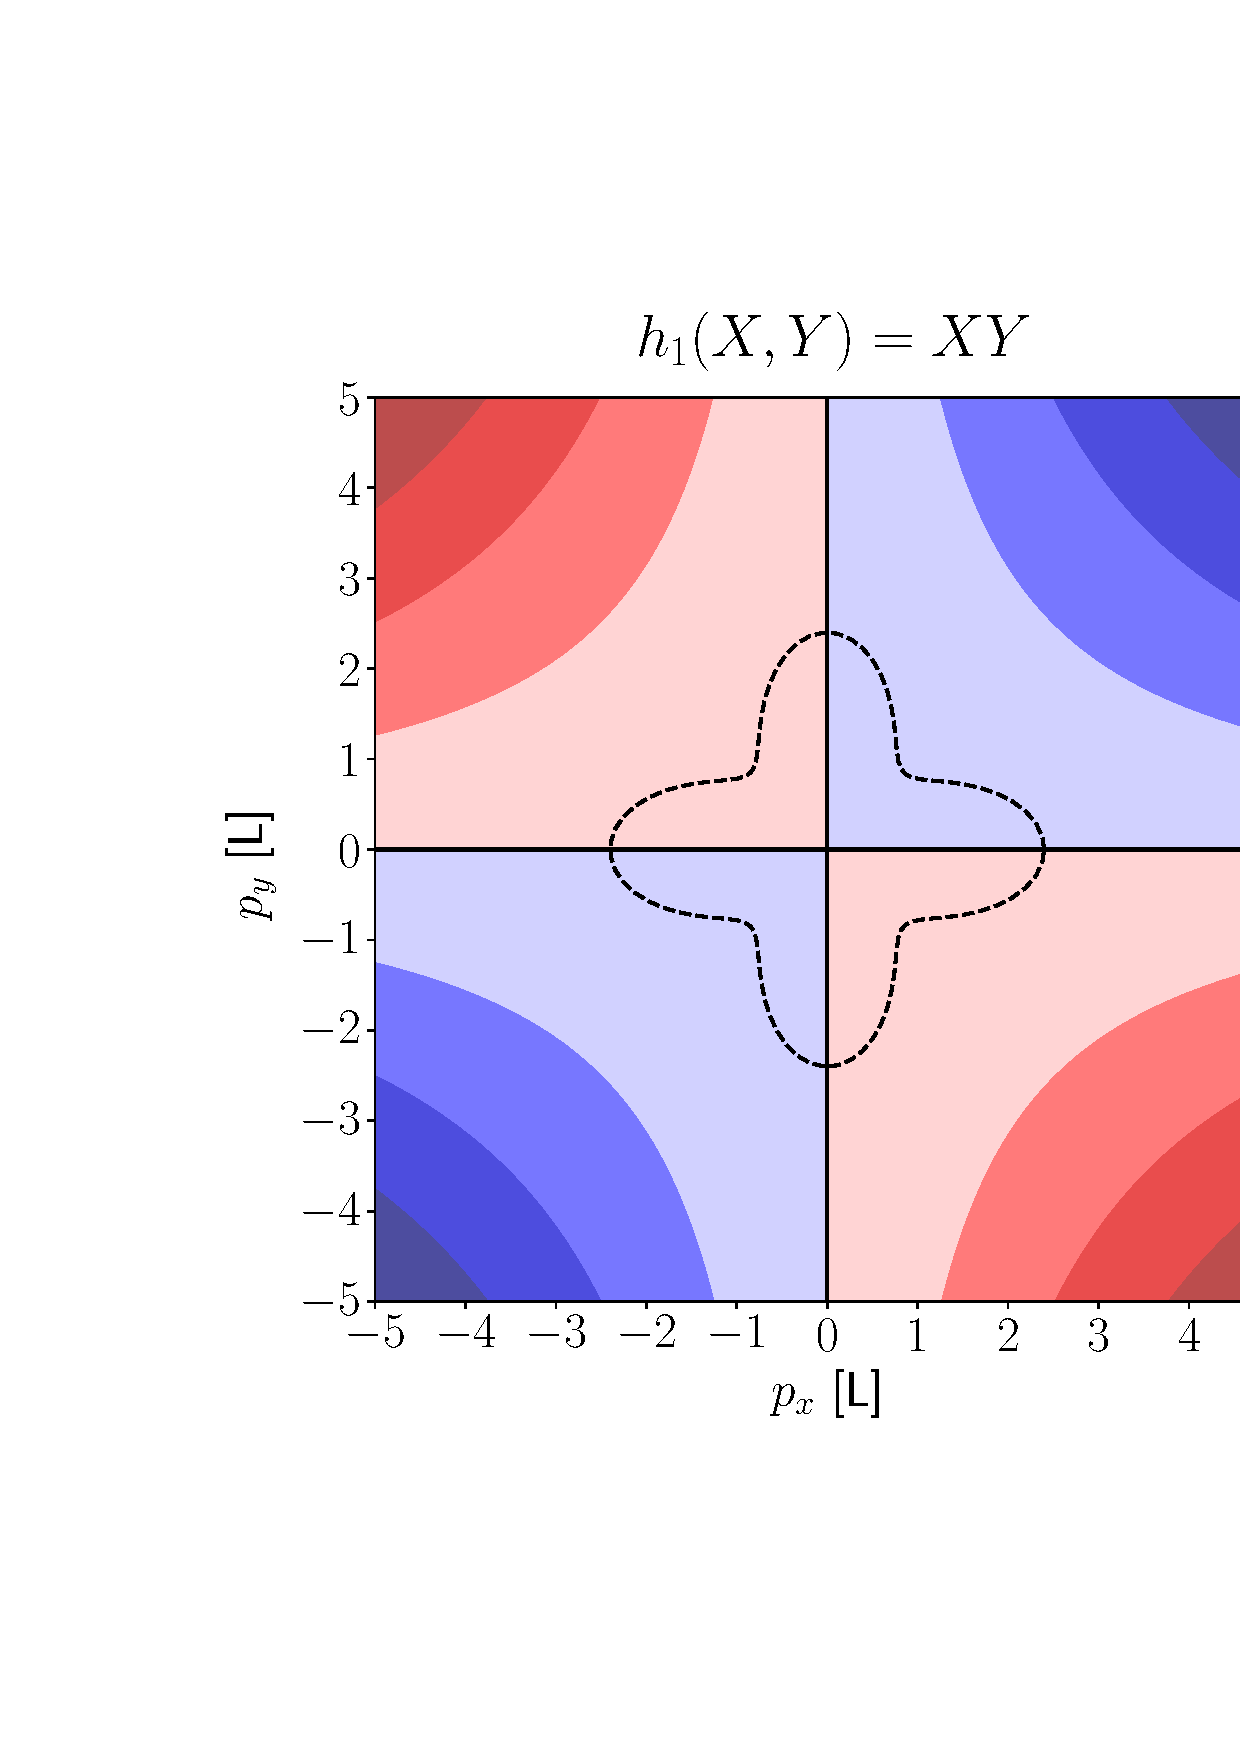
\includegraphics[trim={0 3.5cm 0 4cm}, clip, width=1\columnwidth]{./fig/xy_simetry.png}
    \caption{Contornos de las superficies $h_1$ y $h_2$. En color negro con líneas punteadas se visualizan los límites de la formación y en negro sólido los ejes de simetría.}
    \label{fig: xy_simetry}
\end{figure}

\begin{prop}
\label{prop: l_parallel}
Dada una señal $\sigma$, una formación $x$ y un sistema de coordenadas (X-Y) centrado en $p_c$. Podemos afirmar que, para que la dirección de ascenso $L_\sigma^1(p_c, x)$ sea paralela a $\nabla\sigma(p_c)$, es suficiente que la geometría de dicha formación cumpla simultáneamente las siguientes condiciones:

\begin{enumerate}
    \item Simetría especular con respecto a alguno de los ejes X-Y.
    \item En el interior de cada cuadrante, simetría especular con respecto a alguno de los ejes del sistema de referencia rotado 45º.
\end{enumerate}

\end{prop}

\begin{proof}

Partiendo de (\ref{eq: l1_cont}), es {\color{red}sencillo (evitar este tipo de adjetivos)} identificar las condiciones que tiene que cumplir la geometría de la formación (límites de integración) para que $L_\sigma$ sea paralelo a $\nabla\sigma(p_c)$. Necesitaremos que las integrales sobre $h_1(X,Y) = XY$ y $h_2(X,Y) = X^2 - Y^2$ sean ambas nulas. Véase que, si al integrar sobre $h_2(X,Y)$ obtenemos un valor nulo, entonces las integrales sobre $X^2$ e $Y^2$ serán iguales. Ahora bien, {\color{red} ¿cómo tienen que ser los límites de integración para que estas dos condiciones se cumplan? (no se pueden ahcer preguntas en las demostraciones)} Analicemos cada uno de los casos por separado:



\begin{enumerate}
        \item Supongamos que partimos de una formación con unos límites de integración en el eje X simétricos, como los que se muestran en el primer gráfico de la \autoref{fig: obs_xxyy}. Entonces tendremos que
    \begin{align*}
        \iint_{C} h1(X,Y) \; \mathrm{d}X \mathrm{d}Y 
        & = \frac{1}{2} \int_{-t_\beta}^{t_\beta}\int_{\alpha(X)}^{0} XY \; \mathrm{d}X
        - \frac{1}{2} \int_{-t_\alpha}^{t_\alpha}\int_{0}^{\beta(X)}  XY \; \mathrm{d}X 
        \\
        & = \frac{1}{2} \int_{-t_\beta}^{t_\beta}   X\beta^2(X)  \; \mathrm{d}X
        - \frac{1}{2} \int_{-t_\alpha}^{t_\alpha} X\alpha^2(X) \; \mathrm{d}X
        = 0,
    \end{align*}
    siempre que $\alpha(X)$ y $\beta(X)$ sean funciones pares. Recordemos que, {\color{red}por definición (tiene que estar definido, sino es mejor poner 'acorde a la figura')}, $\alpha(X)<0$ y $\beta(X)>0$, por lo que dichas funciones nunca podrán ser impares.\\
    
    De este modo se puede llegar a la conclusión de que, para que la integral de $h_1(X,Y)$ sobre la formación sea nula, es condición \textit{suficiente} que exista simetría especular con respecto a alguno de los ejes X-Y.\\
    
    \item Para el caso de $h_2(X,Y)$ partiremos de una formación como la que se muestra en el segundo gráfico de la \autoref{fig: obs_xxyy}. Si además dividimos el área $C$ de la formación en cuatro secciones $C_i$ delimitadas por cada uno de los cuadrantes, podemos aprovechar la propiedad aditiva en el dominio de integración para decir que
    
    \begin{equation} \label{eq: ci}
    \iint_{C} h2(X,Y) \; \mathrm{d}X \mathrm{d}Y = \sum^4_{i=1} \iint_{C_i} h2(X,Y) \; \mathrm{d}X \mathrm{d}Y.
    \end{equation}

    De este modo, nos bastará con centrarnos en la integración sobre cada uno de las cuadrantes de forma independiente. Inspirados en las simetrías de $h_2(X,Y)$ (ver \autoref{fig: xy_simetry}), proponemos el cambio de variable $g(\epsilon, \rho) = (\rho + \epsilon, \; \rho - \epsilon)/\sqrt{2}$, equivalente a una rotación de -45º de los ejes X-Y. El teorema del cambio de variable nos dice que
    
    \begin{equation} \label{eq: teorem_cv}
    \int_{A} f(x,y) = \int_{B} (f \circ g) |J_g|. 
    \end{equation}

    Sabiendo que $|J_g| = \begin{bmatrix}\nabla g_1 \\ \nabla g_2 \end{bmatrix} = \sqrt{2}$, entonces tenemos que
    
    \begin{align*}
    \iint_{C_i} h2(X,Y) \; \mathrm{d}X \mathrm{d}Y 
    & = 2 \sqrt{2} \iint_{C_i} \epsilon\rho \; \mathrm{d}\epsilon \mathrm{d}\rho \\
    & = 2 \sqrt{2} \int_{-\pi/4}^{\pi/4}\int_0^{R_i(\phi)} r^3 \cos\phi\sin\phi \; \mathrm{d}r \mathrm{d}\phi \\
    & = \frac{1}{\sqrt{2}} \int_{-\pi/4}^{\pi/4} R_i(\phi)^4 \cos\phi\sin\phi \; \mathrm{d}\phi
    = 0
    \end{align*}
    
    siempre y cuando $R_i(\phi)$ sea una función par. Partiendo de este resultad podemos decir, apoyándonos en (\ref{eq: ci}), que si $R_i(\phi)$ es par $\forall i \in \{1,2,3,4\}$ entonces la integral sobre todo $C$ será nula. En otras palabras, tener una formación tal que, en el interior de cada cuadrante, se guarde simetría especular con respecto a alguno de los ejes del sistema de referencia rotado 45º, será condición suficiente para que la integral de $h_2(X,Y)$ sobre dicha formación sea nula.
\end{enumerate}

\begin{figure}[h]
    \centering
    \includegraphics[trim={0 3cm 0 3.5cm}, clip, width=1\columnwidth]{./fig/obs_xxyy.eps}
    \caption{En el gráfico (a) se muestran los límites, superior $\beta(X)$ (azul) e inferior $\alpha(X)$ (rojo), de una formación con simetría especular respecto al eje Y. Mientras que en (b) se muestra una formación que además, en el interior de cada cuadrante, también cuenta con simetría especular respecto a alguno de los ejes $\epsilon$-$\rho$. Véase que $C_i$ y $R_i(\phi)$ hacen referencia, respectivamente, al dominio de integración dentro del cuadrante $i$ y a la función que delimita dicho dominio. El origen de ambos sistemas de referencia coincide con el centroide de la formación.}
    \label{fig: obs_xxyy}
\end{figure}
\end{proof}


% -----------------------------

% En primer lugar, hemos de identificar que $h_1$ y $h_2$ son el mismo paraboloide hiperbólico, uno rotado 45º con respecto al otro. Las curvas de nivel correspondientes a estas superficies permiten generar toda una familia de hipérbolas. Si nos fijamos por ejemplo en la hipérbola de la curva de nivel $h_2 = 1$ (hipérbola unidad), tenemos que el área encerrada bajo la curva a un lado del eje Y es igual a la encerrada bajo el otro lado. Lo mismo sucede si tomamos $h_2 = -1$, pues es la misma hipérbola rotada 90º con respecto al origen. Teniendo esto en cuenta, es trivial ver que la resta de estas dos áreas nos va a dar un valor nulo.

% Apoyándonos en el razonamiento anterior, y fijándonos en la figura \ref{fig: xy_simetry}, ya somos capaces de mostrar de forma muy intuitiva la respuesta a la pregunta planteada inicialmente. Para que la integral sobre $h_1(X,Y)$ sea nula, necesitaremos que la formación guarde simetría entre los cuadrantes. Si queremos que suceda lo mismo con $h_2(X,Y)$, entonces también requeriremos dentro los cuadrantes de simetría con respecto a los mismos ejes X-Y, pero rotados 45º. Sólo de esta forma lograremos que las contribuciones positivas de volumen a lo largo de toda la región de integración se vean anuladas por las negativas.

La proposición \ref{prop: l_parallel} nos dice que, si la geometría de la formación en el continuo cumple las dos simetrías indicadas, entonces $L_\sigma$ será siempre paralelo a $\nabla\sigma(p_c)$. No obstante, también cabe destacar el caso en el que únicamente se cumple la simetría con respecto a los ejes X e Y, pues entonces tendremos {\color{red}$L_{\sigma_X} \propto \nabla\sigma(p_c)_X$ y $L_{\sigma_Y} \propto \nabla\sigma(p_c)_Y$ (hay que ser más preciso, la componente X de L depende únicamente de la componente X del gradiente... también conviene visualizarlo)}. Dicha propiedad nos permitirá maniobrar al enjambre modificando únicamente su forma, pues tendrá un impacto directo sobre la dirección de ascenso. 

\begin{figure}[!h]
    \centering
    %\includegraphics[width=0.9\columnwidth]{./fig/sim_sqr_maneuvering.eps}
    \caption{\color{red}TFM: grafiquito con simulación chula de los agentes en formación rectangular maniobrando.}
    \label{fig: label}
\end{figure}

{\color{red} Hablar un poco más sobre maniobrabilidad, al fin y al cabo fue una de las motivaciones principales que nos condujo a este resultado :)}